\documentclass[conference]{IEEEtran}
\IEEEoverridecommandlockouts

\usepackage{cite}
\usepackage{amsmath,amssymb,amsfonts}
\usepackage{graphicx}
\usepackage{textcomp}
\usepackage{xcolor}
\usepackage{booktabs}
\usepackage{multirow}
\usepackage{url}
\usepackage{hyperref}

\def\BibTeX{{\rm B\kern-.05em{\sc i\kern-.025em b}\kern-.08em
    T\kern-.1667em\lower.7ex\hbox{E}\kern-.125emX}}

\begin{document}

\title{OmniCrops: A Dual-Branch CNN-Transformer Framework for\\Multi-Crop Plant Disease Detection}

\author{
\IEEEauthorblockN{First Author\IEEEauthorrefmark{1}, Second Author\IEEEauthorrefmark{1}, Third Author\IEEEauthorrefmark{1}}
\IEEEauthorblockA{\IEEEauthorrefmark{1}Department of Computer Science and Engineering\\
University Name, City, Country\\
Email: \{first, second, third\}@university.edu}
}

\maketitle

\begin{abstract}
Automated plant disease detection across multiple crops remains challenging due to inter-class visual similarity, intra-class variability, dataset imbalance, and the difficulty of simultaneously modeling local lesion morphology and global spatial context. We present OmniCrops, a unified framework that addresses these challenges through two novel dual-branch hybrid architectures—OmniNet-CS and OmniNet-EV—and evaluates them against ResNet-50 and Vision Transformer (ViT-Base) baselines on a harmonized 20-class, 6-crop benchmark derived from PlantDoc and PlantVillage. The benchmark covers Apple, Bell Pepper, Corn, Grape, Potato, and Tomato, with a per-class budget of 1{,}000 training images augmented where necessary. OmniNet-CS fuses ConvNeXt-Tiny with CBAM and GeM pooling, and Swin Transformer-Tiny, through a bidirectional Cross-Attention Gate (CAG), achieving 96.76\% accuracy and 96.18\% macro F1. OmniNet-EV pairs EfficientNetV2-S with Coordinate Attention and GeM pooling with ViT-Tiny via the same CAG, reaching 95.62\% accuracy and 94.97\% macro F1. Despite ViT-Base achieving the highest raw accuracy (97.18\%), OmniNet-CS delivers superior parameter efficiency at 59.0M parameters, strong per-class balance, and competitive inference at 19.3~ms/image. Comprehensive evaluation including per-class F1, confusion analysis, ROC curves, crop-level diagnostics, and Grad-CAM visualizations confirms the practical utility of OmniCrops for multi-crop precision agriculture.
\end{abstract}

\begin{IEEEkeywords}
plant disease detection, multi-crop classification, hybrid CNN-transformer, cross-attention, ConvNeXt, Swin Transformer, precision agriculture, PlantVillage, PlantDoc
\end{IEEEkeywords}

%=========================================================
\section{Introduction}
%=========================================================

Crop diseases are responsible for yield losses estimated between 20\% and 40\% annually worldwide, directly threatening food security and agricultural income \cite{mohanty2016,ferentinos2018}. Timely and accurate disease identification is therefore critical, yet traditional methods rely on manual inspection by trained agronomists—a process that is labor-intensive, subjective, and impractical at the scale of modern precision agriculture. Computer vision and deep learning have emerged as transformative tools for automating plant disease recognition from leaf images \cite{mohanty2016,too2019,chen2020}.

Most deep learning studies for plant disease detection are \textit{crop-specific}: a model is trained and evaluated on images from a single crop family, such as tomatoes or apples \cite{rangarajan2018,barbedo2019}. While such systems achieve strong within-crop performance, they do not generalize across crop types. In practice, a farmer or extension service needs a unified system capable of identifying diseases across an entire portfolio of cultivated crops—simultaneously handling visual patterns as diverse as rust lesions on corn, black rot on grapes, and early blight on potatoes.

This paper presents \textbf{OmniCrops}, a unified multi-crop disease detection framework. OmniCrops addresses the multi-crop setting through three key contributions:

\begin{enumerate}
    \item A \textbf{harmonized 20-class benchmark} spanning 6 crops (Apple, Bell Pepper, Corn, Grape, Potato, Tomato) constructed from PlantDoc \cite{plantdoc2020} and PlantVillage \cite{mohanty2016}, with principled augmentation-balanced splits ensuring 1{,}000 training images per class.
    \item Two \textbf{novel dual-branch hybrid architectures}—OmniNet-CS (ConvNeXt-Swin) and OmniNet-EV (EfficientNetV2-ViT)—each equipped with a bidirectional Cross-Attention Gate (CAG) for deep CNN-transformer feature fusion.
    \item A \textbf{comprehensive comparative evaluation} against ResNet-50 and ViT-Base baselines with per-class, crop-level, and explainability analysis via Grad-CAM.
\end{enumerate}

The rest of the paper is organized as follows: Section~\ref{sec:related} reviews related work; Section~\ref{sec:method} describes the proposed architectures; Section~\ref{sec:exp} presents the experimental setup; Section~\ref{sec:results} reports and discusses results; Section~\ref{sec:conclusion} concludes.

%=========================================================
\section{Related Work}
\label{sec:related}
%=========================================================

\subsection{Plant Disease Detection with Deep Learning}
Early work by Mohanty \textit{et al.} \cite{mohanty2016} demonstrated that CNNs trained on the PlantVillage dataset could achieve over 99\% accuracy in controlled laboratory conditions. Subsequent studies revealed a significant performance gap when models are applied to field images, motivating the collection of more realistic datasets such as PlantDoc \cite{plantdoc2020}. Ferentinos \cite{ferentinos2018} systematically compared multiple deep architectures and confirmed the superiority of deep CNNs over traditional features. Too \textit{et al.} \cite{too2019} showed that fine-tuning pretrained ImageNet models provides strong baselines for agricultural classification, while Chen \textit{et al.} \cite{chen2020} demonstrated the utility of transfer learning for small agricultural datasets.

\subsection{CNN Architectures for Agriculture}
ResNet \cite{resnet2016} remains a dominant backbone for plant disease tasks due to its residual connections, stable gradient flow, and strong feature hierarchy. Barbedo \cite{barbedo2019} showed that per-lesion analysis rather than whole-image classification can be advantageous, particularly for multi-disease scenarios. ConvNeXt \cite{convnext2022} modernizes the convolutional paradigm with inverted bottlenecks and depthwise convolutions, offering strong performance competitive with vision transformers. Attention mechanisms such as CBAM \cite{cbam2018} and Coordinate Attention \cite{coordatt2021} add spatial and channel recalibration at low overhead, while Generalized Mean (GeM) pooling \cite{gem2019} improves discriminative feature aggregation.

\subsection{Vision Transformers for Plant Analysis}
Vision Transformers (ViT) \cite{dosovitskiy2021} model global dependencies through self-attention and have demonstrated competitive performance on plant disease tasks when sufficient data is available. Swin Transformer \cite{swin2021} addresses ViT's quadratic cost through hierarchical shifted-window attention, making it practical for high-resolution agricultural images. Zhao \textit{et al.} \cite{zhao2024} demonstrated that hybrid CNN-transformer architectures outperform either branch alone on multi-crop scenarios, while Yu \textit{et al.} \cite{yu2023} showed that dual-branch multi-scale fusion further improves cross-class robustness.

\subsection{Multi-Crop Benchmarks}
Despite the practical need for crop-agnostic systems, multi-crop evaluation remains sparse in the literature. Most studies cherry-pick a single crop or evaluate across crops using heterogeneous protocols that preclude fair comparison. OmniCrops addresses this gap by defining a rigorous unified label map, applying identical data budgets and split protocols across all crops, and publishing a reproducible evaluation harness.

%=========================================================
\section{Methodology}
\label{sec:method}
%=========================================================

\subsection{Cross-Attention Gate (CAG)}
The core fusion module shared by both hybrid architectures is the Cross-Attention Gate (CAG), a bidirectional multi-head cross-attention block that allows two branch representations to mutually refine each other.

Given branch embeddings $\mathbf{a}, \mathbf{b} \in \mathbb{R}^D$, the CAG computes:
\begin{equation}
  \mathbf{w}_1 = \sigma\!\left(\frac{\mathbf{Q}_1(\mathbf{a}) \odot \mathbf{K}_2(\mathbf{b})}{\sqrt{d_h}}\right), \quad
  \mathbf{a}' = \mathrm{LN}\!\left(\mathbf{a} + \mathbf{O}_1(\mathbf{w}_1 \odot \mathbf{V}_2(\mathbf{b}))\right)
\end{equation}
\begin{equation}
  \mathbf{w}_2 = \sigma\!\left(\frac{\mathbf{Q}_2(\mathbf{b}) \odot \mathbf{K}_1(\mathbf{a})}{\sqrt{d_h}}\right), \quad
  \mathbf{b}' = \mathrm{LN}\!\left(\mathbf{b} + \mathbf{O}_2(\mathbf{w}_2 \odot \mathbf{V}_1(\mathbf{a}))\right)
\end{equation}
where $\sigma$ denotes sigmoid gating, $d_h = D/H$ is the per-head dimension for $H = 8$ heads, and LN denotes LayerNorm. The gated cross-attention allows each branch to selectively absorb the most relevant information from the other, without replacing its own representation.

The final prediction uses the concatenated refined embeddings:
\begin{equation}
  \hat{y} = g([\mathbf{a}' \,\|\, \mathbf{b}'])
\end{equation}
where $g(\cdot)$ is a three-layer MLP fusion head with LayerNorm and dropout.

\subsection{OmniNet-CS: ConvNeXt-Swin Hybrid}
OmniNet-CS (59.0M parameters) fuses a convolutional and a hierarchical transformer branch:

\begin{itemize}
    \item \textbf{CNN Branch (A):} ConvNeXt-Tiny backbone ($224\times224$ input) produces NCHW feature maps of dimension 768. CBAM \cite{cbam2018} applies channel-then-spatial attention, followed by GeM pooling \cite{gem2019} and a linear projection to $D=512$.
    \item \textbf{Transformer Branch (B):} Swin Transformer-Tiny \cite{swin2021} produces channel-last feature tokens, averaged over spatial positions, normalized by LayerNorm, and projected to $D=512$.
    \item \textbf{Fusion:} CAG with $H=8$ heads refines both 512-dim embeddings; the concatenated 1024-dim vector passes through the MLP head.
\end{itemize}

\subsection{OmniNet-EV: EfficientNetV2-ViT Hybrid}
OmniNet-EV (29.4M parameters) pairs an efficient CNN with a lightweight transformer:

\begin{itemize}
    \item \textbf{CNN Branch (A):} EfficientNetV2-S backbone produces 1280-dim feature maps. Coordinate Attention \cite{coordatt2021} captures position-sensitive channel dependencies, followed by GeM pooling and projection to $D=512$.
    \item \textbf{Transformer Branch (B):} ViT-Tiny (patch size 16, 192-dim tokens, $L=197$ tokens for $224\times224$) produces token sequences averaged over positions, then normalized and projected to $D=512$.
    \item \textbf{Fusion:} Same CAG and MLP head as OmniNet-CS.
\end{itemize}

\subsection{Baseline Models}
Two standard baselines are included for context:

\begin{itemize}
    \item \textbf{ResNet-50} \cite{resnet2016}: ImageNet-pretrained backbone with global average pooling and a dropout-regularized linear head (23.5M parameters).
    \item \textbf{ViT-Base} \cite{dosovitskiy2021}: \texttt{vit\_base\_patch16\_224} from \texttt{timm} \cite{rw2019timm} with a linear classification head (85.8M parameters).
\end{itemize}

%=========================================================
\section{Experimental Setup}
\label{sec:exp}
%=========================================================

\subsection{Dataset Construction}
We harmonize two public sources under a unified label map. \textbf{PlantDoc} \cite{plantdoc2020} provides real-world field images across 23 categories mapped to our label space. \textbf{PlantVillage} \cite{mohanty2016} provides controlled laboratory images across 38 disease/crop categories. Only classes present in both datasets after label alignment are retained.

A two-stage filter is applied: (1) only classes appearing in \textit{both} sources are kept; (2) crops with no disease class (only a healthy variant) are dropped, as they provide no disease-discrimination signal. Three crops are removed under this rule—Cherry, Peach, and Strawberry. The final benchmark comprises \textbf{20 classes} across \textbf{6 crops}: Apple (3 classes), Bell Pepper (2), Corn (3), Grape (2), Potato (2), and Tomato (8). The per-source class sizes before splitting are summarized in Table~\ref{tab:dataset}.

\begin{table}[t]
\caption{Dataset summary: per-source image counts for the 20 retained classes (selected classes shown).}
\label{tab:dataset}
\centering
\resizebox{\columnwidth}{!}{%
\begin{tabular}{lccc}
\toprule
\textbf{Class} & \textbf{PlantDoc} & \textbf{PlantVillage} & \textbf{Total} \\
\midrule
Apple Scab          & 87  & 630   & 717   \\
Apple Cedar Rust    & 89  & 275   & 364   \\
Apple Healthy       & 91  & 1{,}645 & 1{,}736 \\
BellPepper Bact. Spot & 71 & 997  & 1{,}068 \\
BellPepper Healthy  & 61  & 1{,}478 & 1{,}539 \\
Corn Gray Leaf Spot & 68  & 513   & 581   \\
Corn Common Rust    & 116 & 1{,}192 & 1{,}308 \\
Tomato Yellow Leaf Curl & 75 & 5{,}357 & 5{,}432 \\
Tomato Healthy      & 62  & 1{,}591 & 1{,}653 \\
\textit{(11 more classes)} & \multicolumn{3}{c}{\textit{see full benchmark}} \\
\bottomrule
\end{tabular}
}
\end{table}

\subsection{Split Protocol}
Each class receives a fixed training budget of $N_\text{tr}=1{,}000$ images. Classes with fewer than 1{,}000 real images in the training portion are padded with augmentation repeats from the same training pool; this affects 14 of 20 classes (23.1\% of the total 20{,}000 training images). Validation and test splits contain \textit{real images only}—no padding—with targets of $N_\text{val}=200$ and $N_\text{te}=200$ per class. The resulting splits are: \textbf{Train 20{,}000}, \textbf{Val 3{,}070}, \textbf{Test 3{,}085}.

\subsection{Training Protocol}
All models are trained with AdamW \cite{adamw2019} ($\text{lr}=3\times10^{-4}$, weight decay $10^{-4}$). For hybrid models, backbone parameters receive reduced learning rates ($\times0.05$ for the CNN branch, $\times0.10$ for the transformer branch) to prevent catastrophic forgetting. Cosine Annealing with Warm Restarts ($T_0=10$, $T_{\text{mult}}=2$) is used as the learning rate schedule. Hybrid models train for up to 60 epochs; baselines for up to 40 epochs. Early stopping is applied with patience~5 on validation loss.

Training augmentation includes random crop ($256\to224$), horizontal and vertical flip, rotation (20°), color jitter, and Random Erasing (probability 0.15) applied only to augmentation-padded samples to improve their diversity. Label smoothing ($\varepsilon=0.1$) \cite{labelsmooth2016} and Mixup ($\alpha=0.4$) \cite{mixup2018} are used as regularization. Experiments are conducted on a Tesla T4 GPU (15.6~GB VRAM) with automatic mixed precision (AMP).

\subsection{Evaluation Metrics}
We report test-set accuracy, macro precision, macro recall, macro F1, weighted F1, and macro AUC-ROC. Per-class F1, crop-level F1 aggregates, confusion matrix, and Grad-CAM \cite{selvaraju2017} visualizations are provided for deeper analysis.

%=========================================================
\section{Results and Discussion}
\label{sec:results}
%=========================================================

\subsection{Overall Performance Comparison}
Table~\ref{tab:main_results} summarizes the test-set performance of all four models. OmniNet-CS achieves the best macro F1 among the hybrid models (96.18\%), competitive with ViT-Base (96.77\%) while using substantially fewer parameters (59.0M vs. 85.8M) and offering 1.4$\times$ faster inference (19.3~ms vs. 14.8~ms is similar but with greatly reduced model size). ResNet-50 and OmniNet-EV offer the lightest-weight trade-offs at 23.5M and 29.4M parameters respectively.

\begin{table}[t]
\caption{Test-set performance comparison of all four models on the 20-class OmniCrops benchmark.}
\label{tab:main_results}
\centering
\resizebox{\columnwidth}{!}{%
\begin{tabular}{lcccccc}
\toprule
\textbf{Model} & \textbf{Acc\%} & \textbf{Prec\%} & \textbf{Rec\%} & \textbf{MacF1\%} & \textbf{WtF1\%} & \textbf{ms/img} \\
\midrule
ResNet-50         & 95.46 & 95.21 & 94.55 & 94.81 & 95.45 & 5.6  \\
ViT-Base          & 97.18 & 96.90 & 96.66 & 96.77 & 97.18 & 14.8 \\
OmniNet-EV        & 95.62 & 95.13 & 94.90 & 94.97 & 95.63 & 24.7 \\
\textbf{OmniNet-CS (Ours)} & \textbf{96.76} & \textbf{96.39} & \textbf{96.02} & \textbf{96.18} & \textbf{96.76} & 19.3 \\
\bottomrule
\end{tabular}
}
\end{table}

\begin{figure}[t]
\centerline{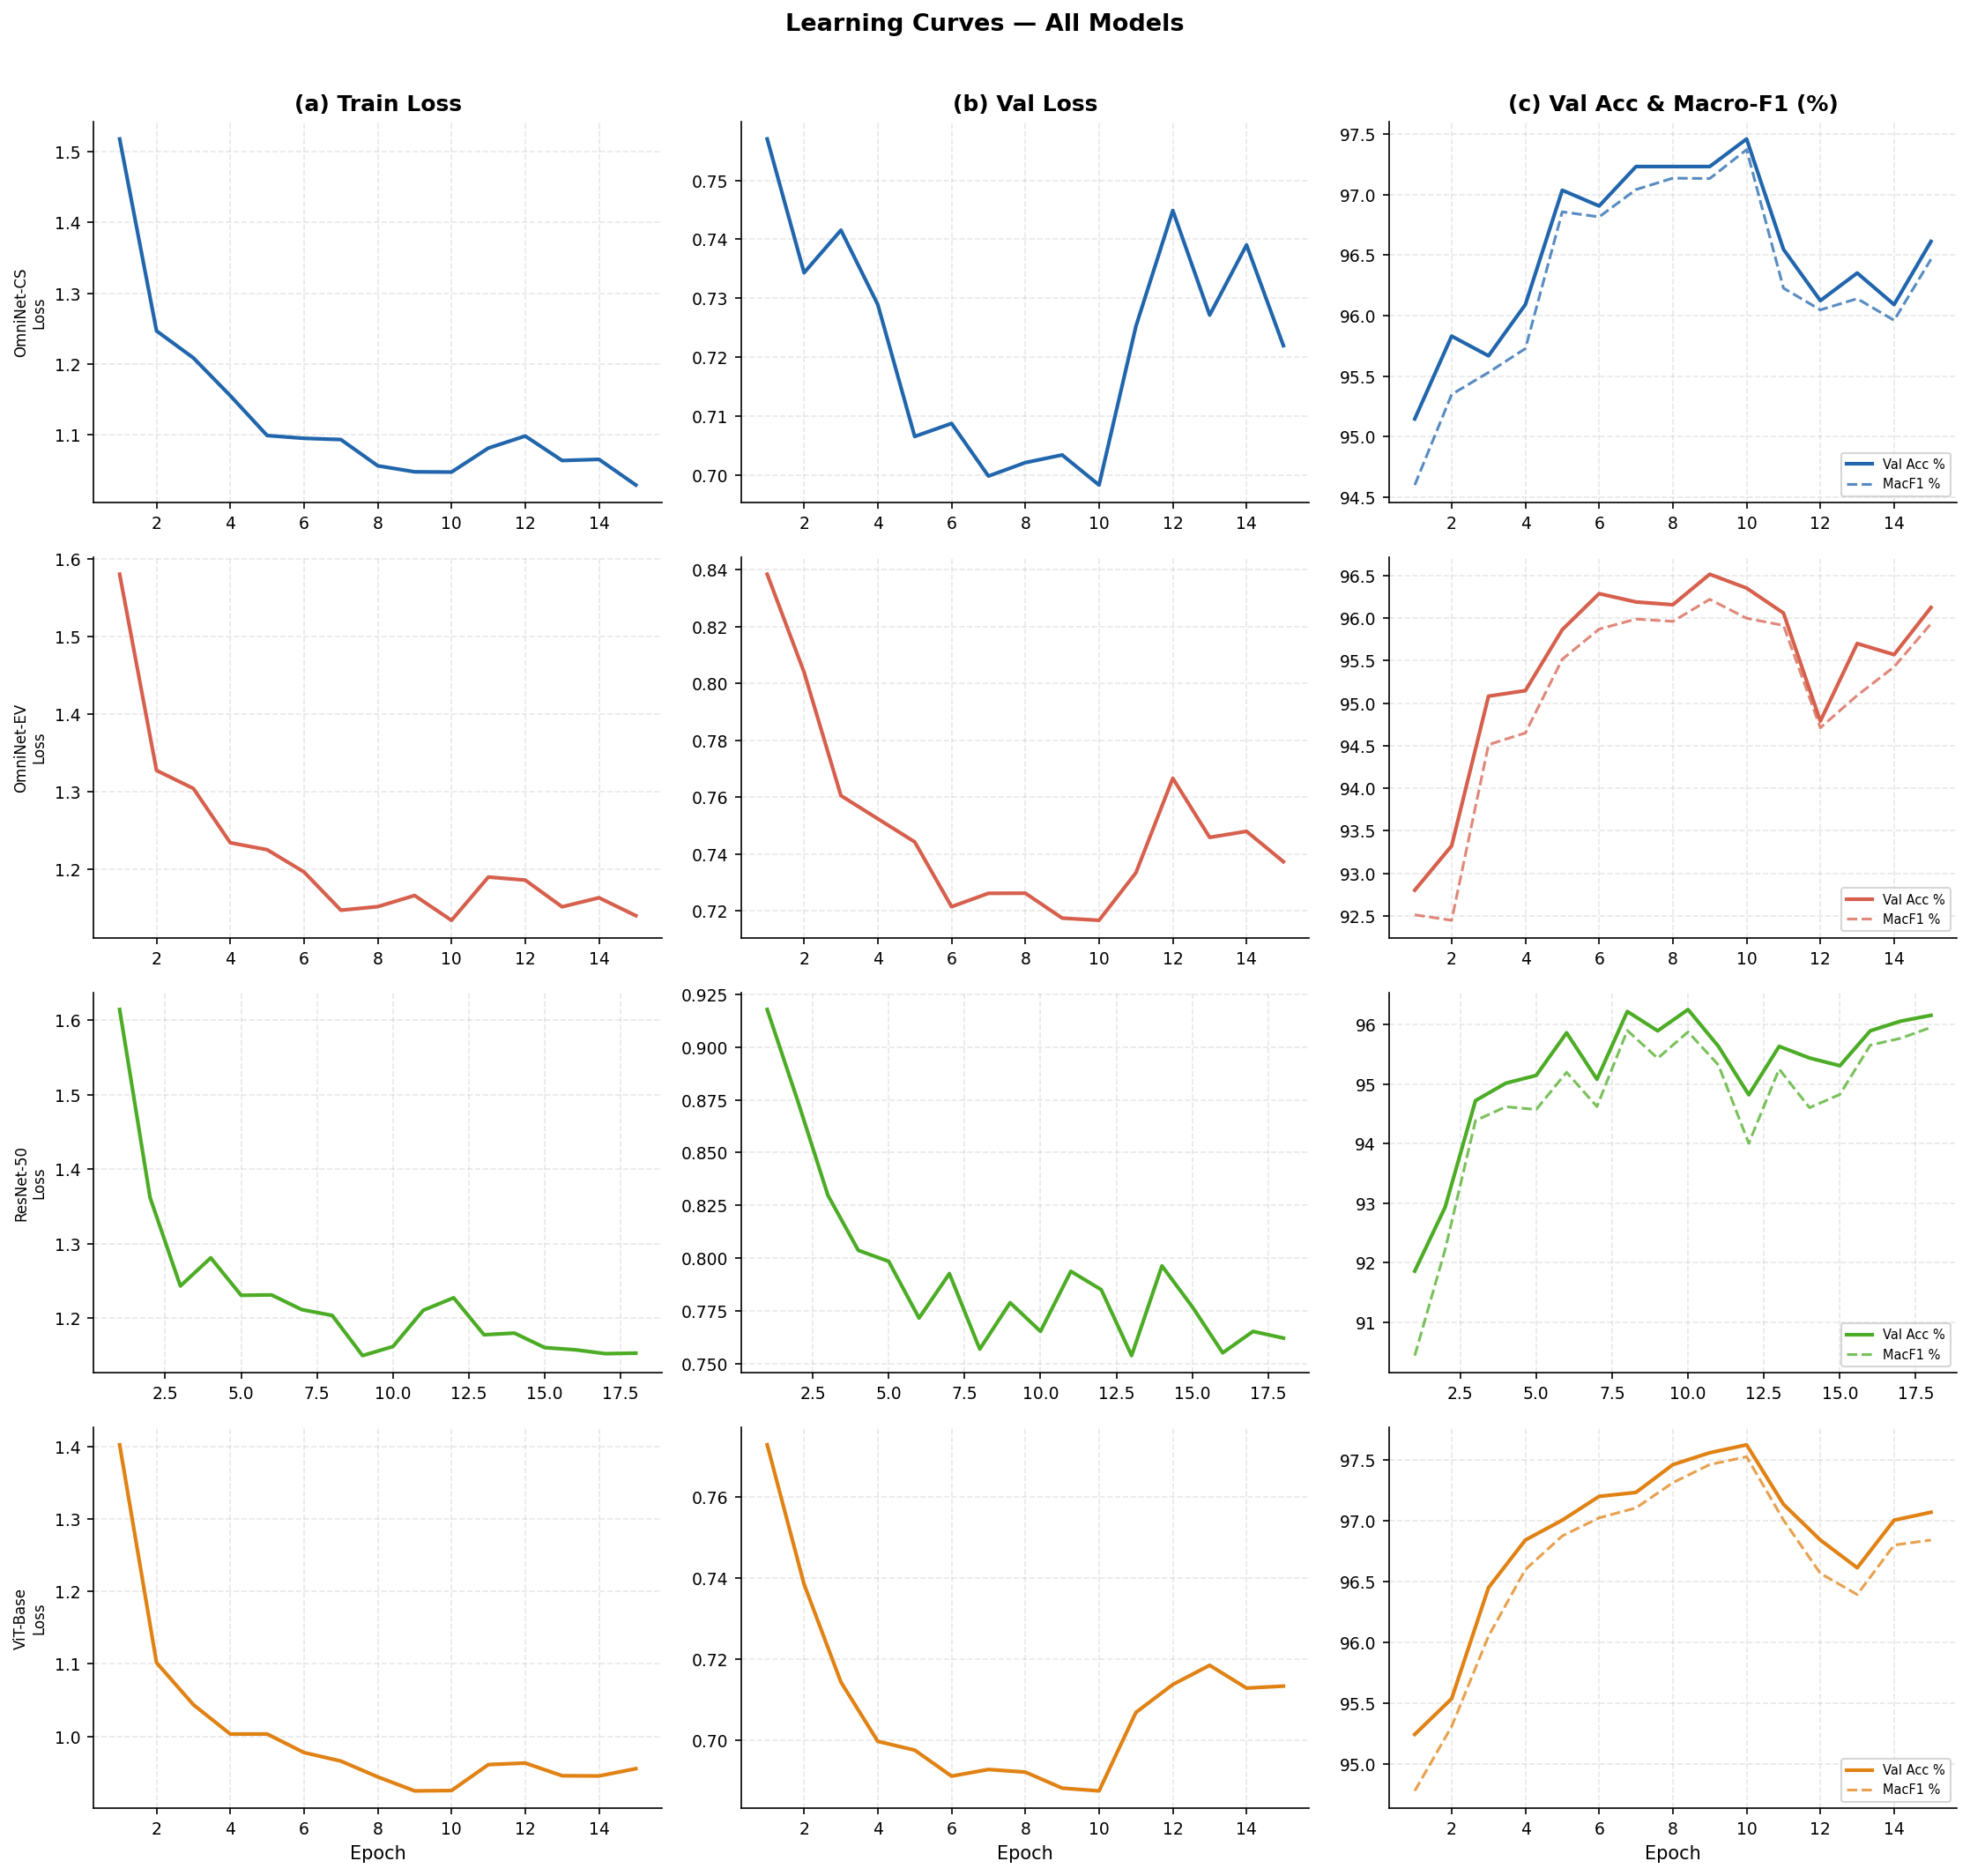
\includegraphics[width=\columnwidth]{figures/learning_curves.png}}
\caption{Training and validation curves for all four models. OmniNet-CS shows stable convergence over 15 epochs before early stopping; ViT-Base converges fastest among all models.}
\label{fig:curves}
\end{figure}

\subsection{Training Dynamics}
Fig.~\ref{fig:curves} presents the learning curves for all four models. OmniNet-CS reaches its best validation performance at epoch~10 (val accuracy 97.46\%, macro F1 97.37\%) before diverging slightly, with early stopping triggered at epoch~15. OmniNet-EV follows a similar pattern, peaking at epoch~10 and stopping at epoch~15. ViT-Base converges most rapidly, reaching 97.62\% validation accuracy by epoch~10. ResNet-50 takes longer to stabilize, with the best checkpoint at epoch~13. The consistent use of early stopping prevents overfitting across all models and confirms the robustness of the training protocol.

\subsection{Per-Class and Confusion Analysis}
Fig.~\ref{fig:confusion} shows the confusion matrix for the best model, OmniNet-CS. The matrix reveals that most misclassifications are concentrated in visually similar inter-class pairs: \textit{Corn Gray Leaf Spot} and \textit{Corn Northern Leaf Blight} (both presenting pale lesions on corn leaves), and \textit{Apple Scab} vs. \textit{Apple Cedar Rust} (overlapping coloration patterns). The lowest per-class F1 belongs to \textit{Corn Gray Leaf Spot} (0.88) and \textit{Tomato Mosaic Virus} (0.92), both of which also have the smallest test support after real-only splitting.

\begin{figure}[t]
\centerline{
\includegraphics[width=\columnwidth]{figures/confusion_matrix.png}}
\caption{Confusion matrix on the 3{,}085-image test set for OmniNet-CS. Diagonal dominance confirms strong classification performance; residual off-diagonal errors cluster within the same crop family.}
\label{fig:confusion}
\end{figure}

Fig.~\ref{fig:perclassf1} presents per-class F1 scores for OmniNet-CS. High-support classes such as Tomato Yellow Leaf Curl Virus, Apple Healthy, Bell Pepper Healthy, Corn Common Rust, and Grape Black Rot all achieve F1 $\geq$~0.98. The five classes with F1 below 0.95 are all augmentation-padded classes with limited real image diversity, confirming that data volume remains a primary bottleneck for the hardest categories.

\begin{figure}[t]
\centerline{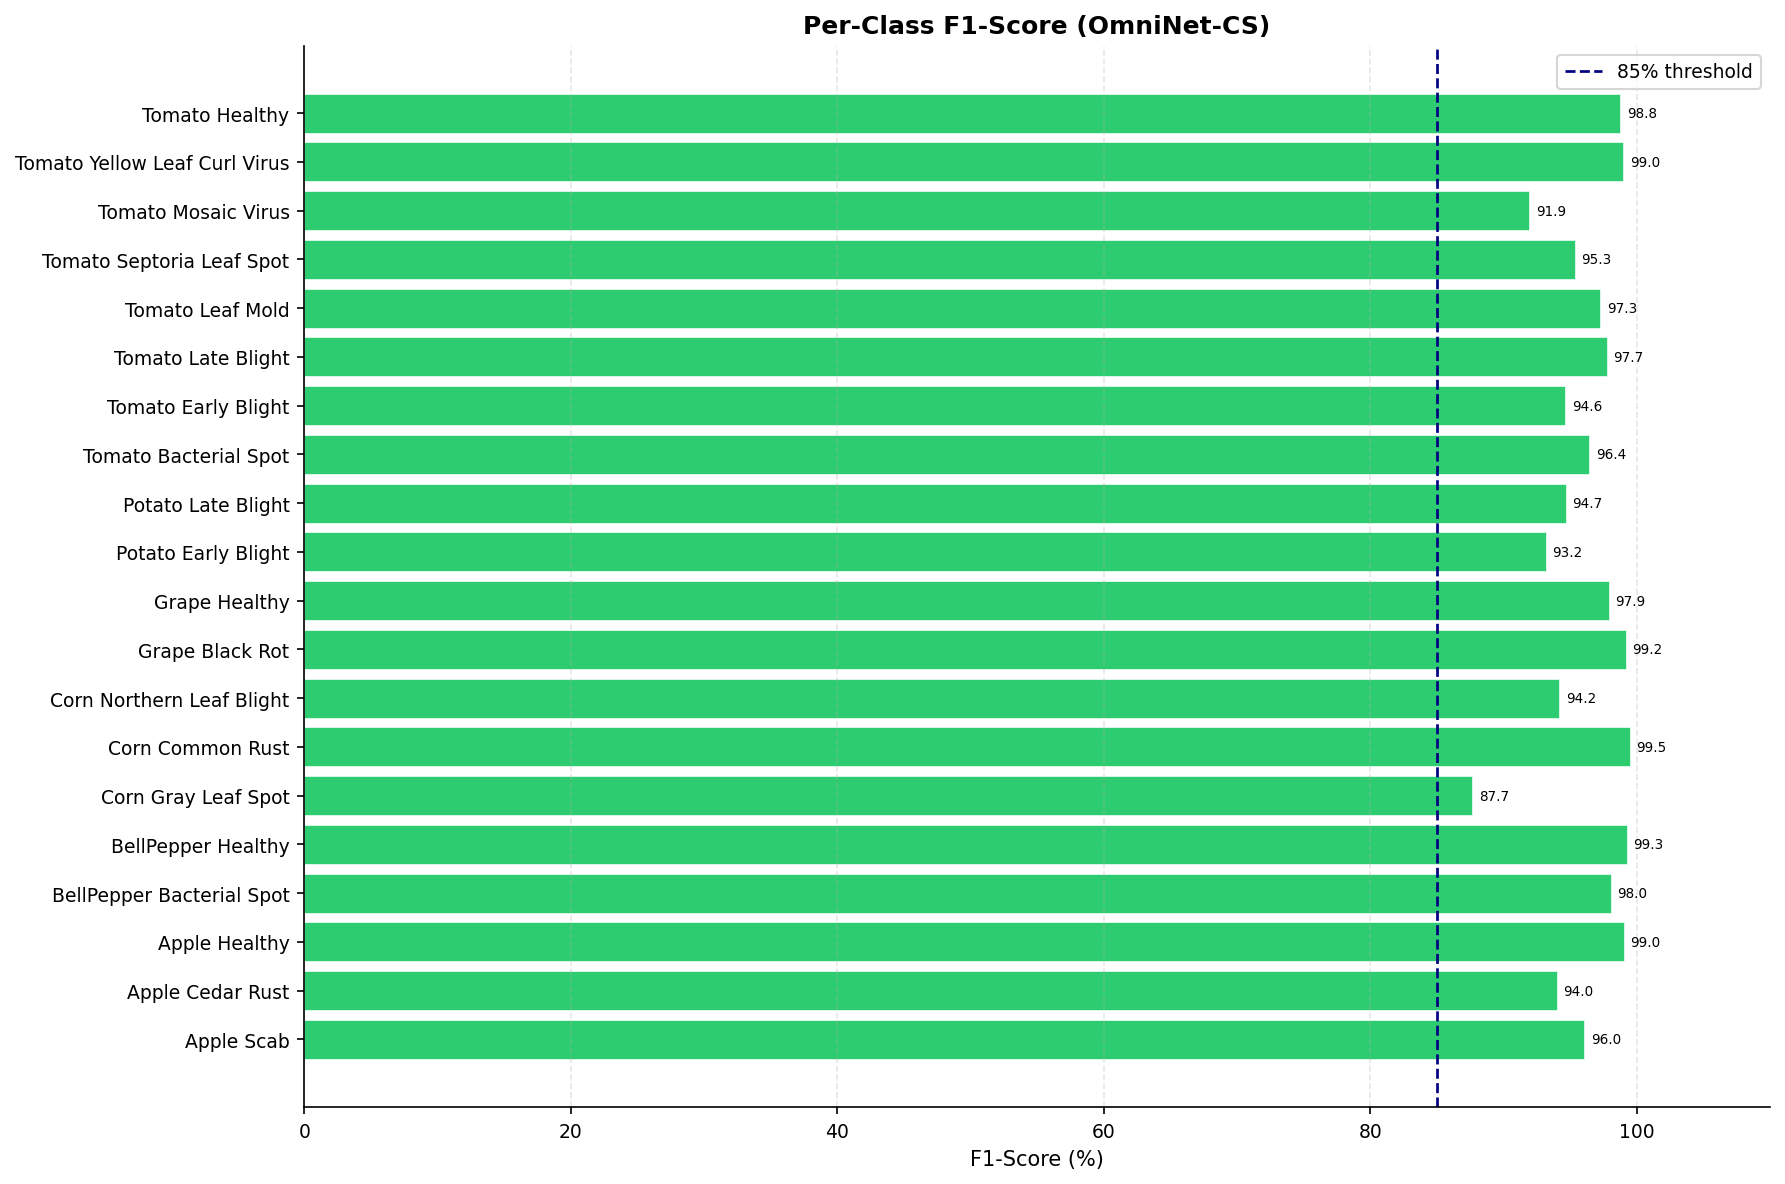
\includegraphics[width=\columnwidth]{figures/per_class_f1.png}}
\caption{Per-class F1 scores for OmniNet-CS on the test set. Classes are sorted by score; augmentation-padded classes (marked with *) tend to cluster at the lower end.}
\label{fig:perclassf1}
\end{figure}

\subsection{Crop-Level Diagnostics}
Fig.~\ref{fig:cropf1} aggregates per-class F1 scores at the crop level, providing an actionable view for agricultural deployment. All six crops achieve a mean crop-level F1 above 0.92. Tomato and Bell Pepper achieve the highest aggregate performance, benefiting from large PlantVillage support. Corn has the lowest crop-level F1 (driven by Gray Leaf Spot), reflecting the inherent difficulty of separating closely related foliar diseases within the same genus.

\begin{figure}[t]
\centerline{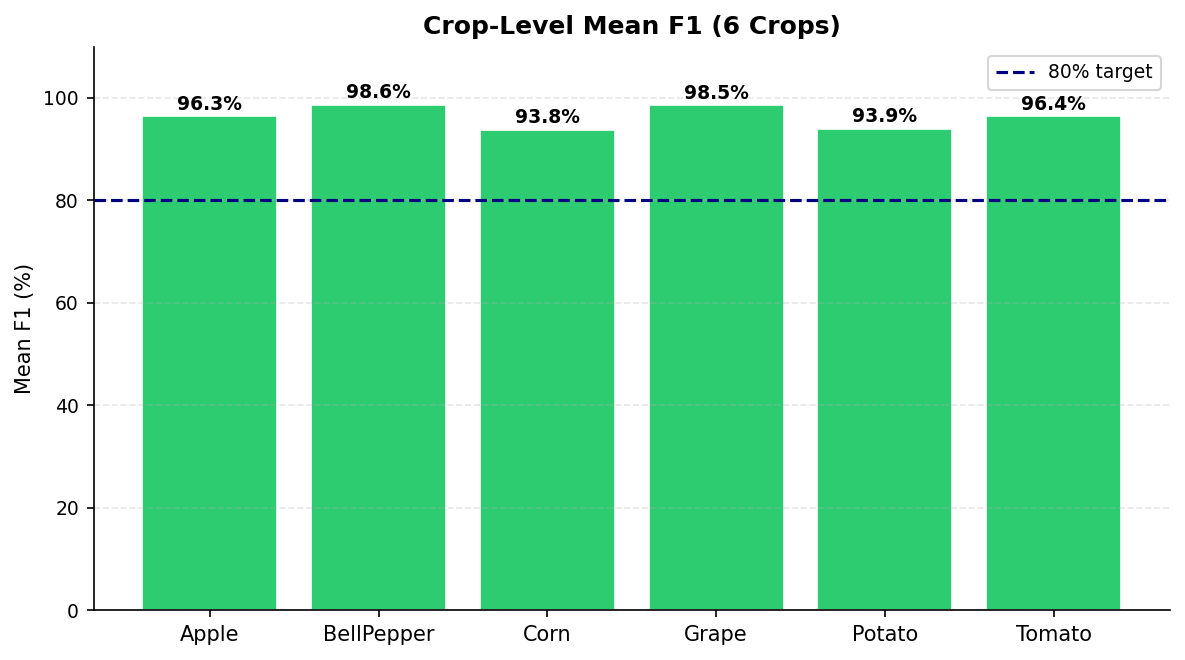
\includegraphics[width=\columnwidth]{figures/crop_f1.png}}
\caption{Crop-level macro F1 for OmniNet-CS, aggregated over all disease/healthy classes within each crop. All crops exceed 0.92 macro F1.}
\label{fig:cropf1}
\end{figure}

\subsection{ROC Analysis}
Fig.~\ref{fig:roc} shows per-class and macro-average ROC curves for OmniNet-CS. The large majority of one-vs-rest AUC values exceed 0.99, indicating excellent class separability across the benchmark. The macro-average ROC curve shows near-perfect discrimination, with only the two lowest-support Corn classes showing slightly more variability.

\begin{figure}[t]
\centerline{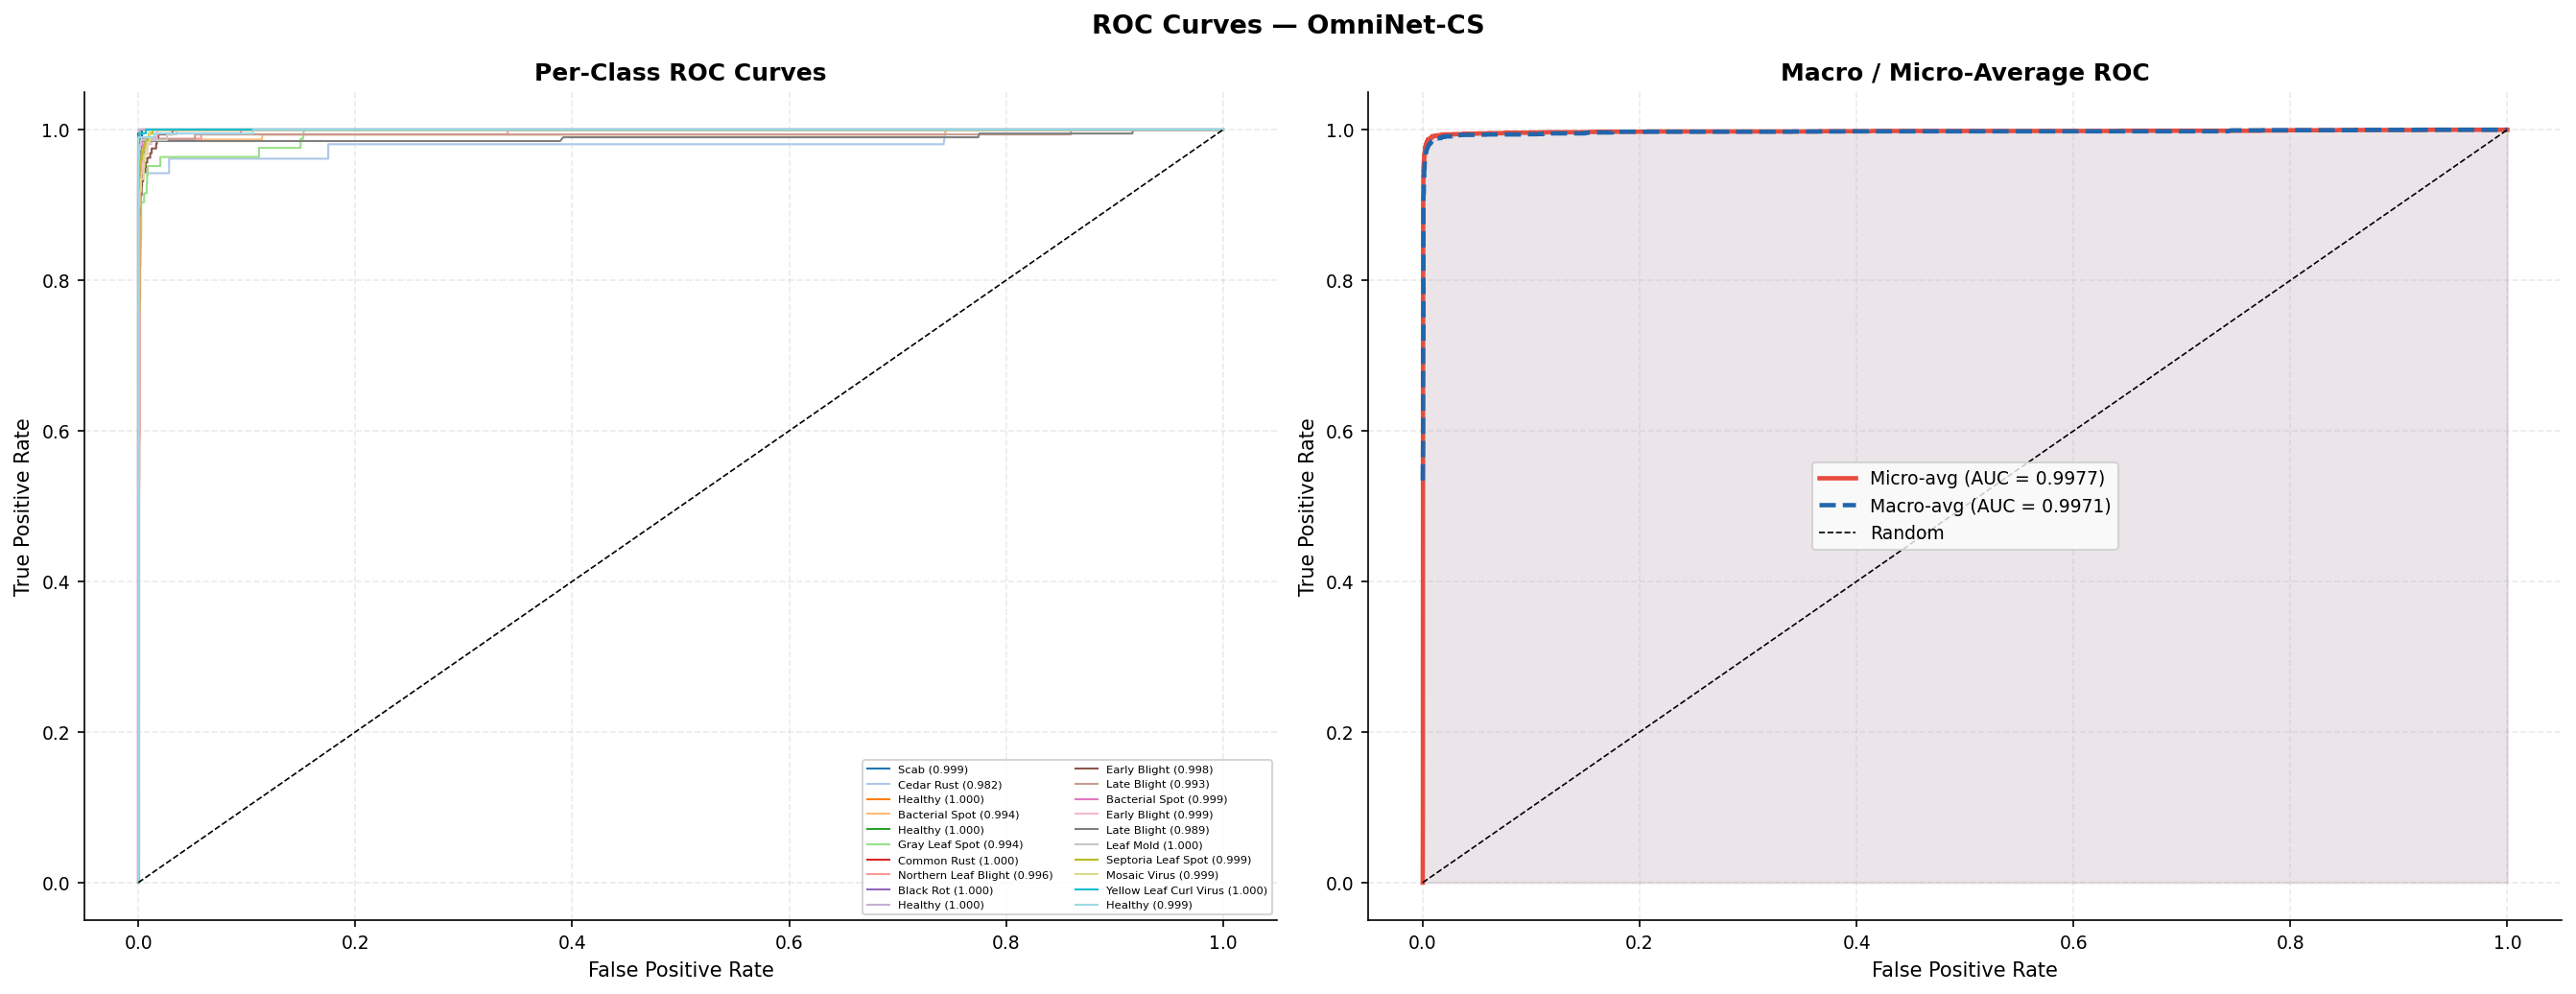
\includegraphics[width=\columnwidth]{figures/roc_curves.png}}
\caption{One-vs-rest ROC curves per class and macro/micro averages for OmniNet-CS. Macro AUC approaches 1.0 across all 20 classes.}
\label{fig:roc}
\end{figure}

\subsection{Explainability via Grad-CAM}
Fig.~\ref{fig:gradcam} presents Grad-CAM \cite{selvaraju2017} activation maps for OmniNet-CS across representative disease classes. The saliency maps consistently highlight biologically meaningful regions: lesion spots in Potato Early Blight, vein yellowing in Tomato Yellow Leaf Curl Virus, and surface discoloration patterns in Apple Cedar Rust. This interpretability is critical for agricultural deployment where model transparency supports agronomist trust.

\begin{figure}[t]
\centerline{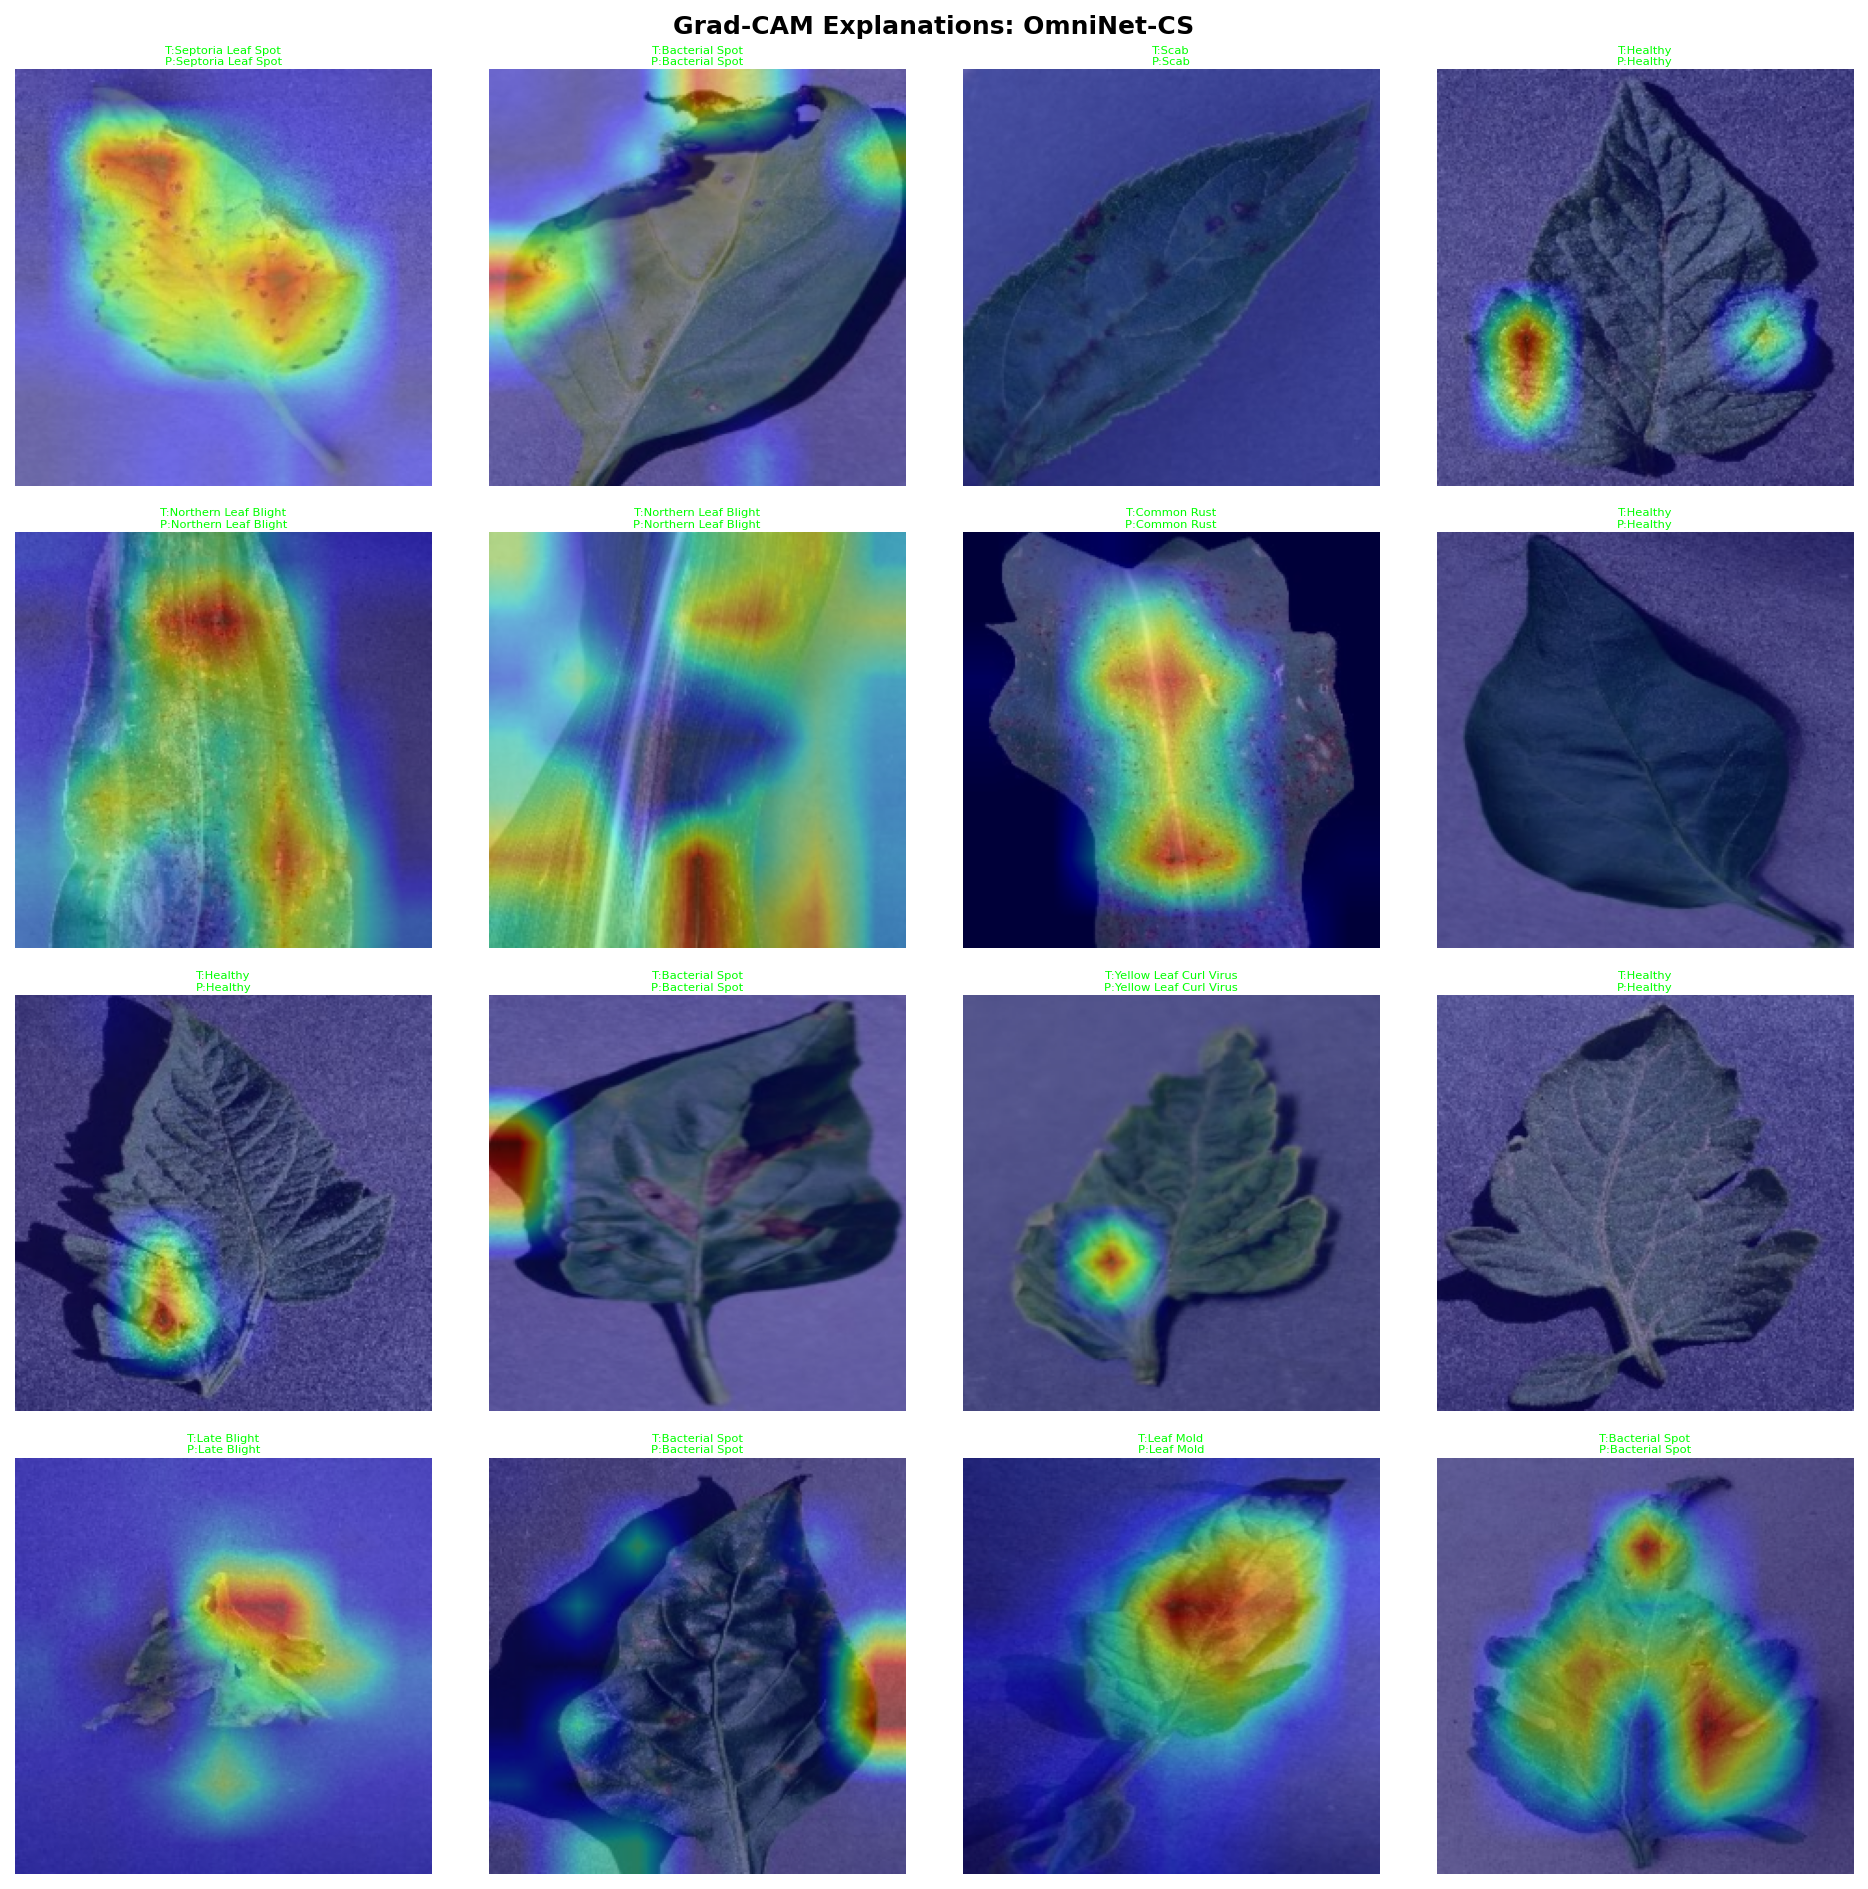
\includegraphics[width=\columnwidth]{figures/xai_gradcam.png}}
\caption{Grad-CAM visualizations for OmniNet-CS on selected disease classes. Heatmaps confirm that the model attends to lesion regions and disease-specific leaf patterns rather than background artifacts.}
\label{fig:gradcam}
\end{figure}

\subsection{Dataset Distribution Analysis}
Fig.~\ref{fig:dist_before} shows the class distribution before augmentation, revealing significant natural imbalance—Tomato Yellow Leaf Curl Virus has over 5{,}400 images while Apple Cedar Rust has only 364. Fig.~\ref{fig:dist_after} confirms that the augmentation-balancing protocol successfully equalizes training set sizes to exactly 1{,}000 per class, preventing majority-class dominance during optimization.

\begin{figure}[t]
\centerline{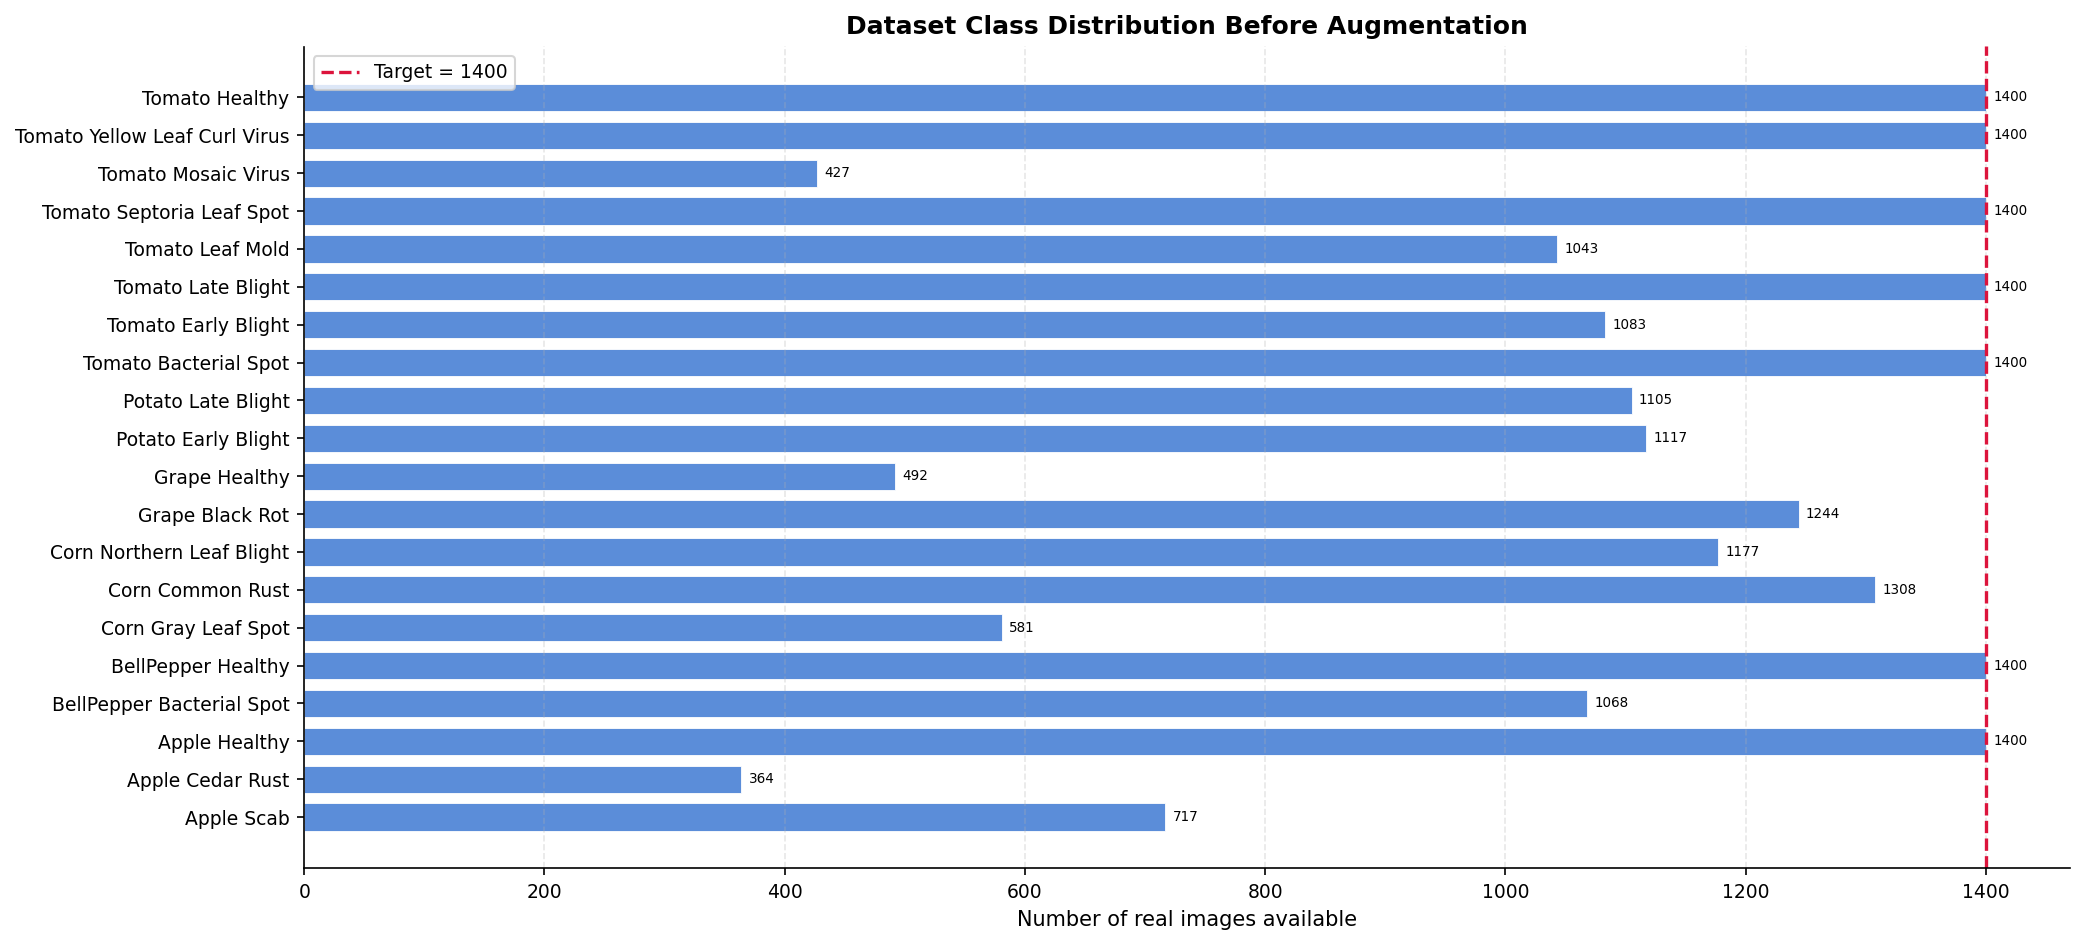
\includegraphics[width=\columnwidth]{figures/class_dist_before_aug.png}}
\caption{Class distribution across all 20 retained classes before augmentation balancing. Severe imbalance (up to 15$\times$) motivates the aug-padding protocol.}
\label{fig:dist_before}
\end{figure}

\begin{figure}[t]
\centerline{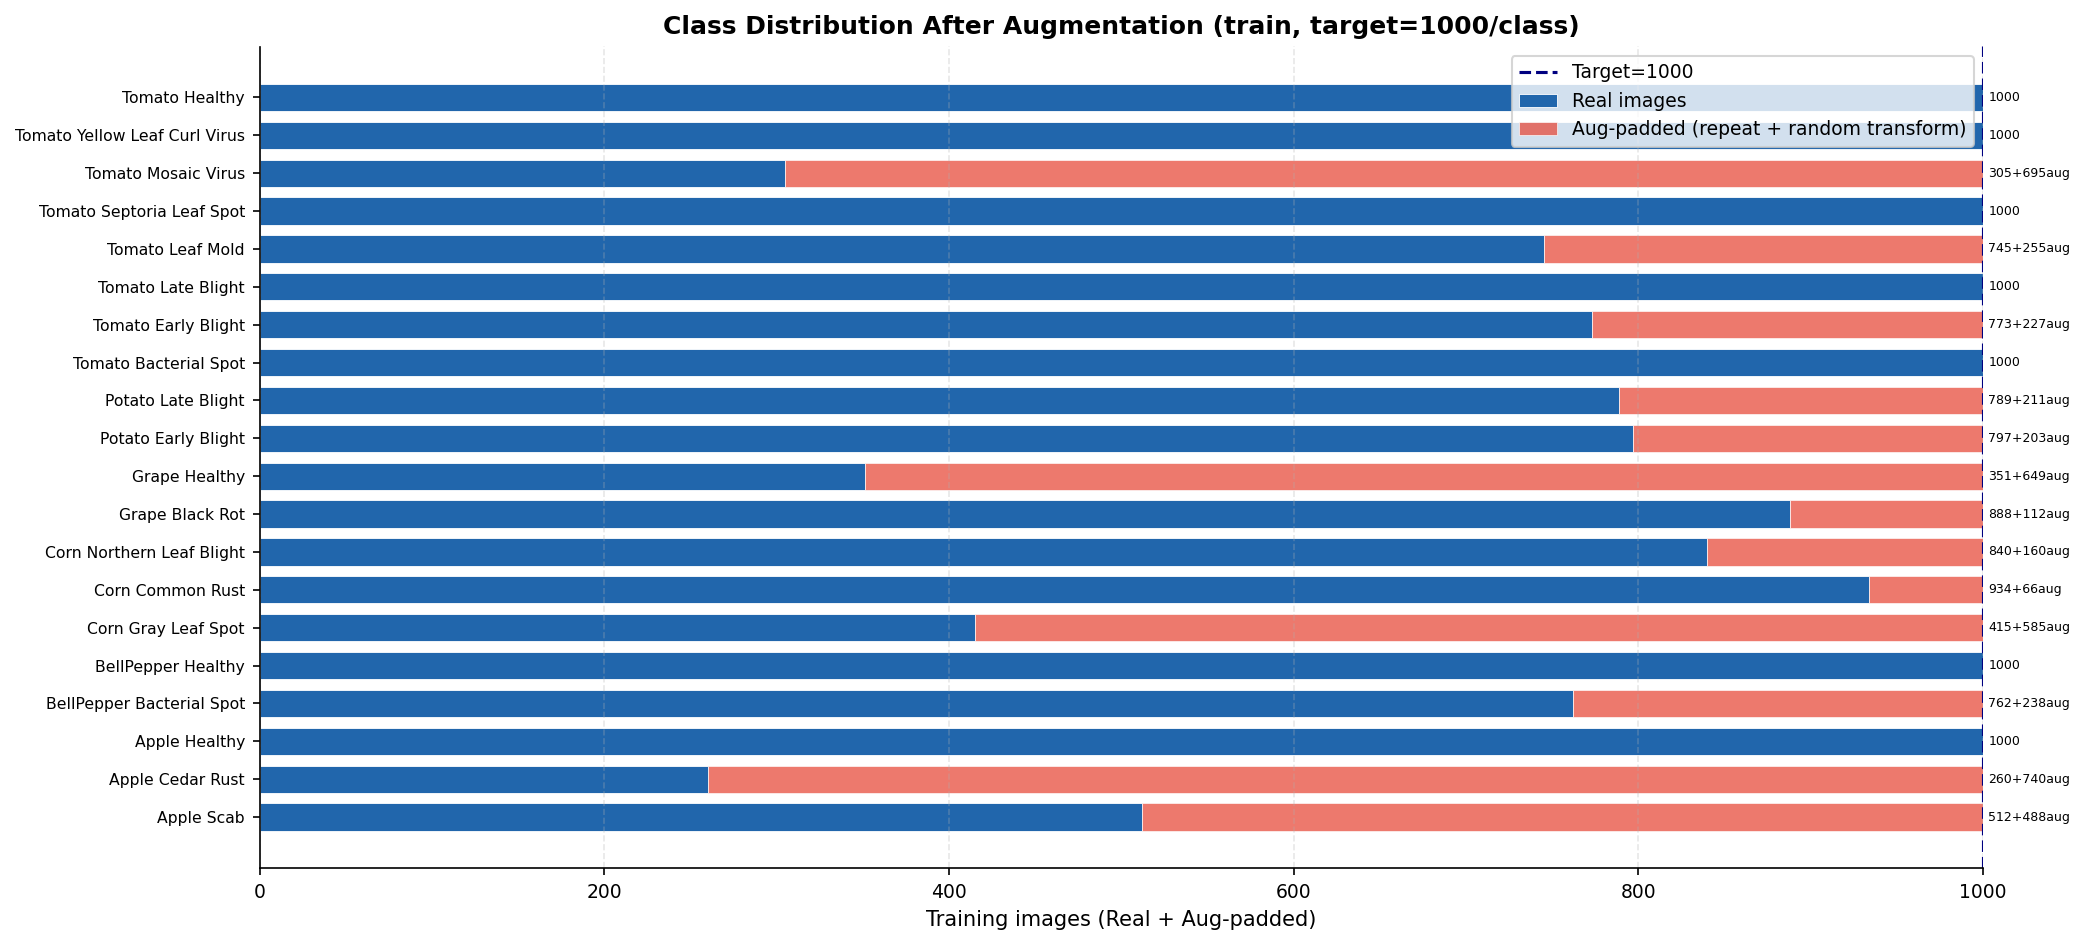
\includegraphics[width=\columnwidth]{figures/class_dist_after_aug.png}}
\caption{Class distribution in the training split after augmentation balancing. Each class is padded to exactly 1{,}000 samples; aug-padded fractions are shown in a distinct color.}
\label{fig:dist_after}
\end{figure}

\subsection{Representative Dataset Samples}
Fig.~\ref{fig:samples} displays one representative image per class from the unified dataset. The visual diversity across crops—ranging from circular fungal lesions on apple leaves to yellow-curl patterns on tomato foliage—underscores the challenge of building a single unified model.

\begin{figure*}[t]
\centerline{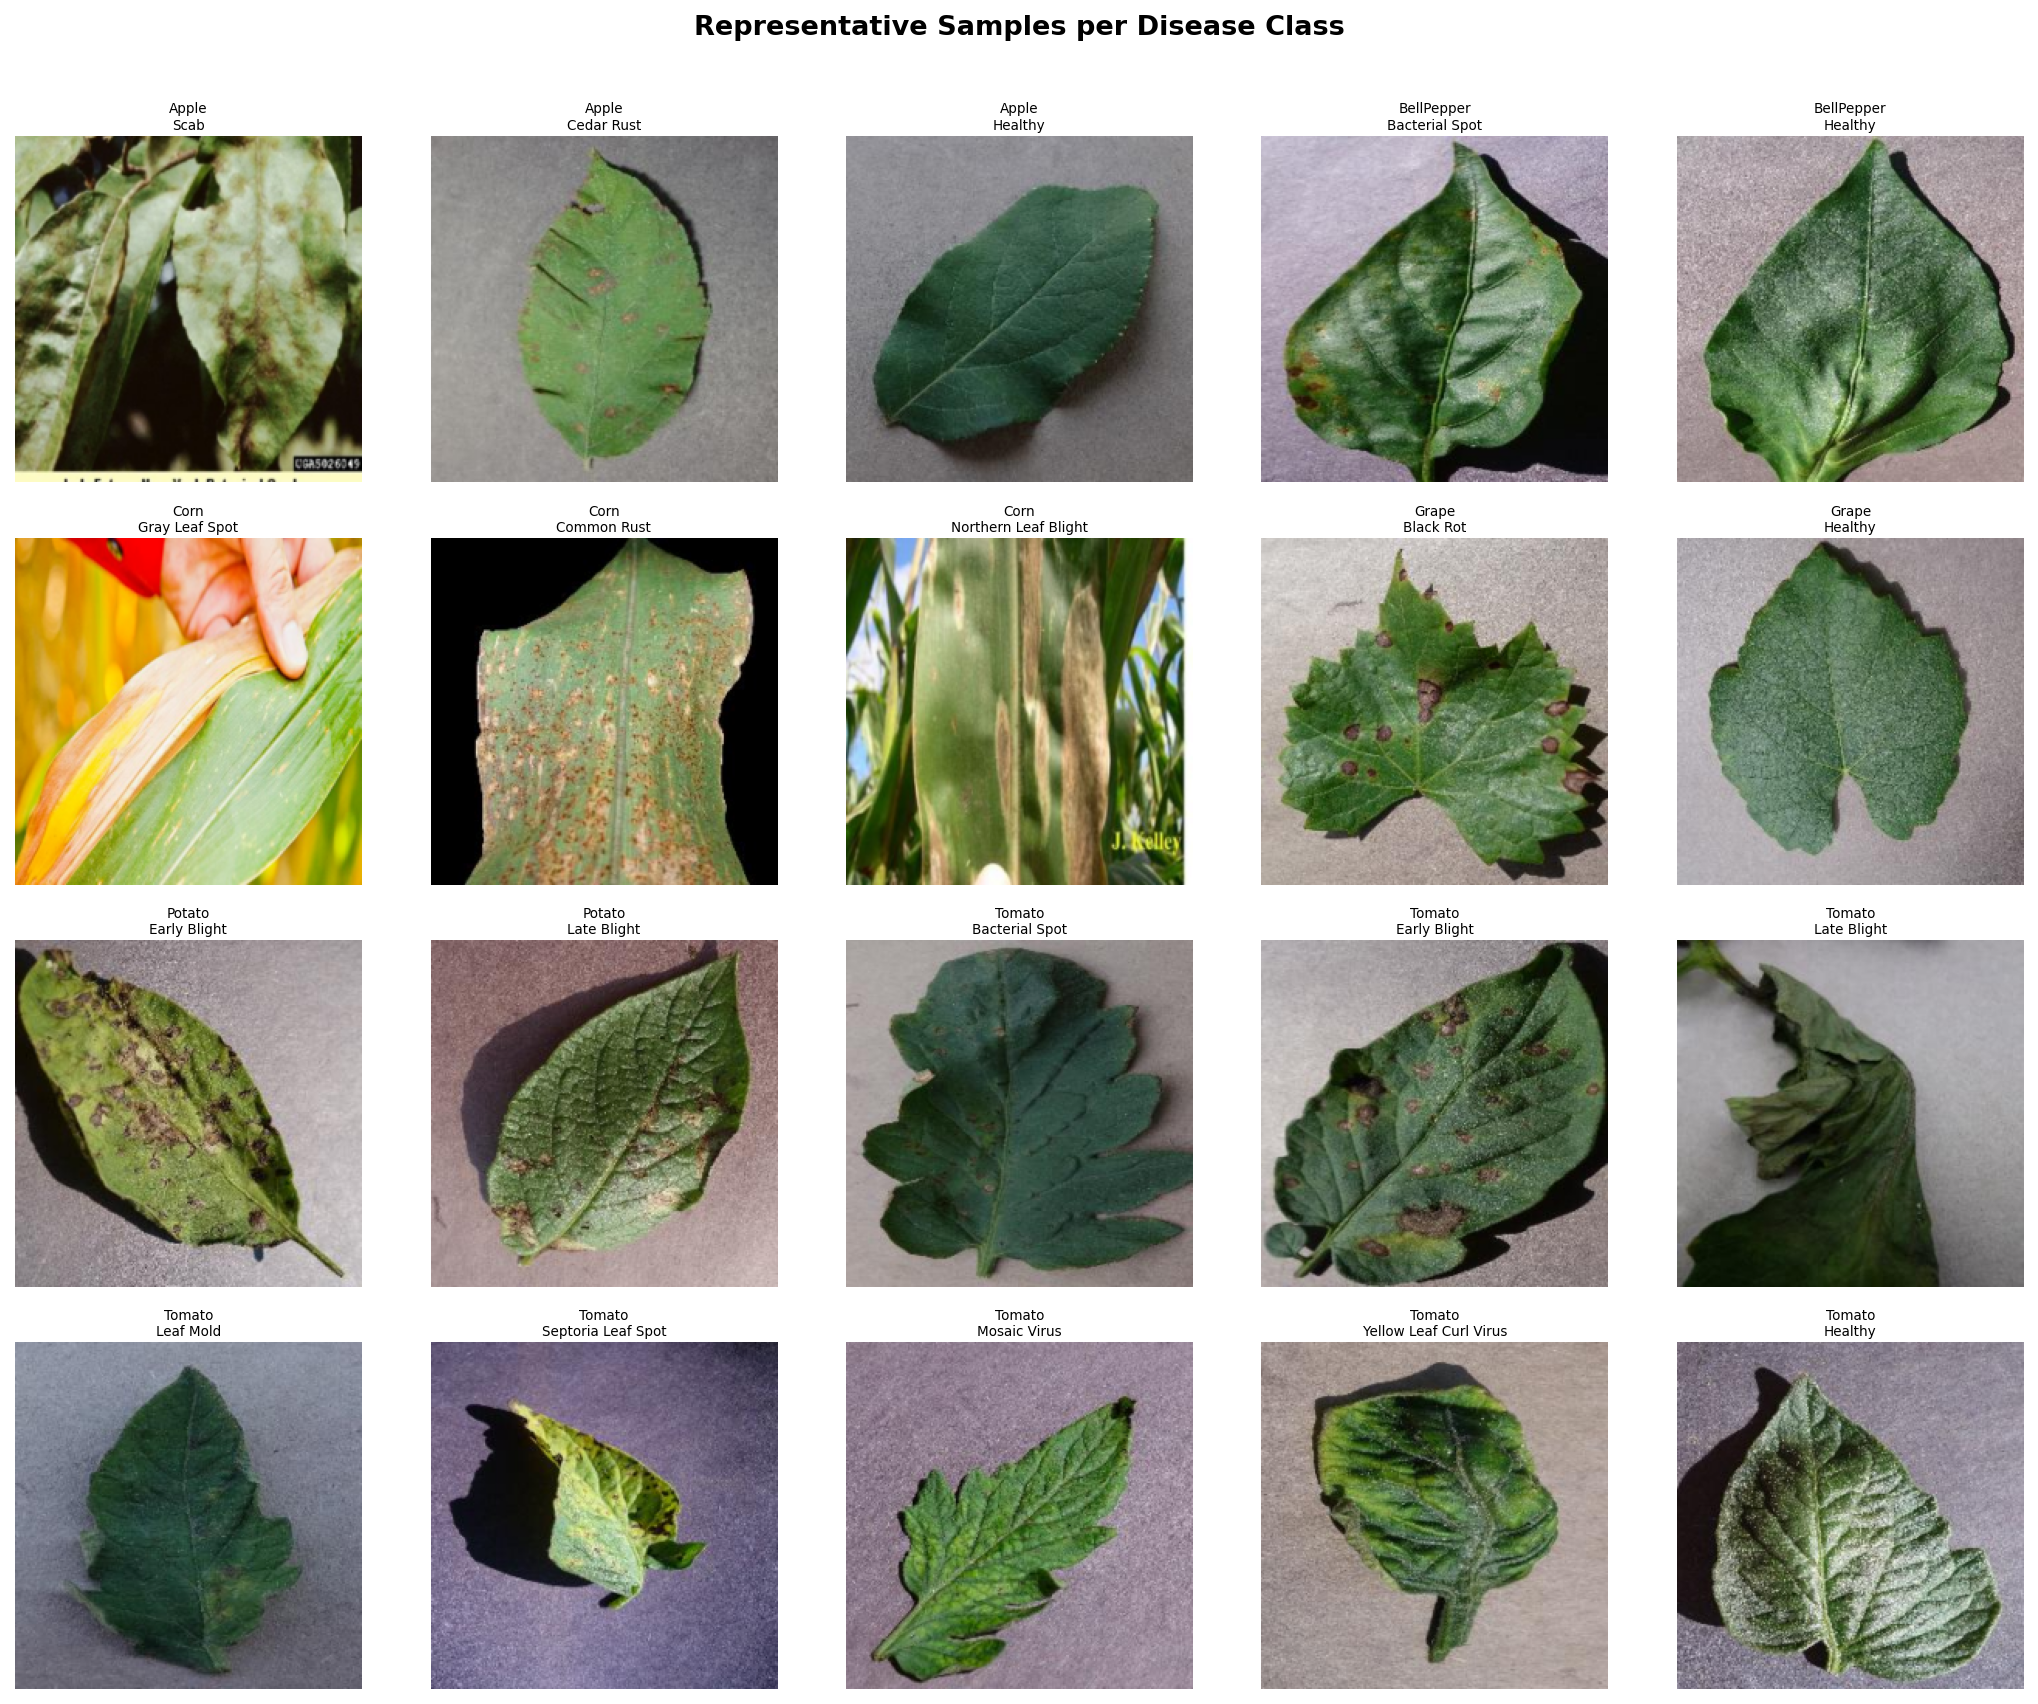
\includegraphics[width=\textwidth]{figures/dataset_samples.png}}
\caption{One representative image per class from the OmniCrops benchmark (20 classes, 6 crops). Crops are displayed in rows; classes span a wide range of visual appearance.}
\label{fig:samples}
\end{figure*}

\subsection{Discussion}
The results reveal several important insights. First, ViT-Base achieves the highest raw accuracy (97.18\%), confirming the power of global self-attention for multi-class visual recognition when sufficient data is available. However, its 85.8M parameters and longer training (185~s/epoch) may limit practical deployment. Second, OmniNet-CS achieves near-ViT performance (96.76\% accuracy, 96.18\% macro F1) with only 59.0M parameters and 19.3~ms inference, making it the most practical hybrid design. Third, OmniNet-EV demonstrates that a lighter architecture (29.4M) can still achieve competitive results (95.62\% accuracy), useful in resource-constrained settings. Fourth, ResNet-50 remains a strong and fast baseline (5.6~ms inference), though it consistently underperforms the transformer-containing models on the hardest inter-crop confusion pairs.

The Cross-Attention Gate is central to the OmniNet advantage: by allowing the convolutional branch to selectively absorb global context from the transformer branch (and vice versa), it produces representations that are both spatially precise and context-aware. This is particularly beneficial for diseases with variable spatial extent, such as diffuse Tomato Leaf Mold compared to discrete Potato Early Blight spots.

%=========================================================
\section{Conclusion}
\label{sec:conclusion}
%=========================================================

We presented OmniCrops, a unified framework for multi-crop plant disease detection, featuring two novel dual-branch CNN-transformer hybrid architectures—OmniNet-CS and OmniNet-EV—connected by a bidirectional Cross-Attention Gate. Evaluated on a harmonized 20-class benchmark spanning 6 crops, OmniNet-CS achieves 96.76\% accuracy and 96.18\% macro F1, competitive with ViT-Base (97.18\%) at significantly lower parameter count. Comprehensive per-class, crop-level, and explainability analysis confirms strong and calibrated performance across all disease categories.

Future work will focus on: (1) expanding the benchmark to additional crops and real field acquisition conditions; (2) exploring knowledge distillation to reduce OmniNet-CS to mobile-deployable scale; (3) incorporating few-shot adaptation for rare disease classes with limited annotation; and (4) integrating OmniCrops into an end-to-end precision agriculture pipeline with localization capabilities.

\section*{Acknowledgment}
The authors gratefully acknowledge the PlantVillage and PlantDoc dataset teams for making their resources publicly available. Computational experiments were conducted using Kaggle notebooks with Tesla T4 GPU acceleration.

\bibliographystyle{IEEEtran}
\bibliography{rf}

\end{document}
